\documentclass[conference]{IEEEtran}

\usepackage{amsmath,amssymb}
\usepackage{booktabs}
\usepackage{array}
\usepackage{cite}
\usepackage{url}
\usepackage{microtype}
\usepackage{pgfplots}
\pgfplotsset{compat=1.16}
\usepackage[hidelinks]{hyperref}

\newcommand{\sigmoid}{\sigma}

\begin{document}

\title{Toxion: Multitask Toxicity Prediction on Tox21 with\\
Fingerprint Baselines, Message Passing and Hybrid Fusion}

\author{Aditya Kishore Singh}

\maketitle

\begin{abstract}
Tox21 is a standard benchmark for predicting twelve in-vitro toxicity endpoints from molecular structure. It is small, has many missing labels, is strongly class-imbalanced, and rewards generalization to new scaffolds. We audit and analyze the dataset (7{,}823 molecules after cleaning, 17.1\% of labels missing, positive rates from 2.9\% to 16.2\%), study its chemical space and scaffold structure, and give the theory of the models, losses and metrics used. A multitask linear baseline on Morgan fingerprints, trained with an optimizer and epoch count chosen on validation data, reaches a test ROC-AUC of 0.654 on one scaffold split, against 0.902 on its training data. The gap and the structure of the data motivate richer features and a graph model fused with fingerprints. Results are preliminary: one split and one seed.
\end{abstract}

\begin{IEEEkeywords}
toxicity prediction, Tox21, molecular fingerprints, message passing, multitask learning, scaffold split
\end{IEEEkeywords}

\section{Introduction}
Computational toxicity models rank chemicals by likely activity in assays to prioritize testing. The Tox21 program screened about ten thousand environmental chemicals and drugs, and the data became a benchmark through the Tox21 Data Challenge~\cite{huang2016tox21}. The endpoints are \emph{in-vitro assay outcomes}, not direct measures of human toxicity.

Three properties make the task hard. Labels are missing for many molecule--endpoint pairs, and ``not tested'' must not be treated as ``inactive''. Actives are rare, so accuracy misleads. Random splits let near-duplicate molecules fall on both sides, so evaluation on held-out scaffolds is more realistic~\cite{yang2019analyzing}.

The research question is whether adding fixed fingerprint, descriptor and alert features to a learned graph embedding improves multitask prediction at this scale, and for which endpoints. Fingerprint models can match learned representations on small data~\cite{yang2019analyzing}, so a fingerprint baseline is the bar to clear. This report covers the data audit and analysis, the feature design, the theory, and the baseline; the graph and fusion models are planned.

\section{Literature Review}
\textbf{Benchmark.} The Tox21 challenge asked for models of twelve assays from structure; the winners, from nearly 400 submissions, all exceeded 80\% accuracy~\cite{huang2016tox21}. DeepTox, the challenge winner, used multitask deep networks and reported better results than naive Bayes, SVMs and random forests~\cite{mayr2016deeptox}. MoleculeNet standardized Tox21 with fixed splits and metrics and found learnable representations broadly best, with dataset-dependent caveats~\cite{wu2018moleculenet}.

\textbf{Features.} Morgan (extended-connectivity) fingerprints hash circular atom neighborhoods into bit vectors~\cite{rogers2010ecfp}; the Tanimoto coefficient is a standard and well-performing similarity for them~\cite{bajusz2015tanimoto}. Bemis--Murcko scaffolds reduce a molecule to its ring systems and linkers~\cite{bemis1996murcko}.

\textbf{Graph models.} Message-passing networks combine a message function, a node update and a readout; the edge-network message with GRU update and Set2Set readout was introduced for quantum-chemistry targets~\cite{gilmer2017mpnn,cho2014gru,vinyals2016order}. Sum-aggregation message passing is at most as discriminative as the Weisfeiler--Lehman test~\cite{xu2019gin}. A large benchmark of directed message passing reports that evaluation must account for scaffold overlap, that fingerprint models can win on small datasets (up to about 1{,}000 training molecules), and that adding computed molecule-level features to the learned representation helps~\cite{yang2019analyzing}; the last finding motivates fusion here.

\textbf{Training and evaluation.} Adam and AdamW are standard optimizers~\cite{kingma2015adam,loshchilov2019adamw}; the precision--recall plot is preferred to ROC under heavy imbalance~\cite{saito2015pr}; and temperature scaling is a simple post-hoc calibration~\cite{guo2017calibration}.

\textbf{Gap.} This work proposes no new architecture. It asks, under scaffold splits, where a from-scratch message-passing network plus fingerprint fusion helps and where it does not, per endpoint.

\section{Dataset and Data Quality}
We use the MoleculeNet distribution of Tox21~\cite{wu2018moleculenet}: a SMILES string and twelve binary endpoints (NR-AR, NR-AR-LBD, NR-AhR, NR-Aromatase, NR-ER, NR-ER-LBD, NR-PPAR-gamma, SR-ARE, SR-ATAD5, SR-HSE, SR-MMP, SR-p53), with labels 1, 0 or missing.

\textbf{Cleaning.} Each SMILES is parsed and canonicalized with RDKit~\cite{rdkit}; unparseable rows are dropped; label cells are coerced to numbers; duplicate canonical SMILES are counted (the first is kept) and conflicting duplicates are logged; missing labels stay NaN, never zero. Zero-filling would turn untested pairs into inactives and bias every model and metric.

\textbf{Audit.} Table~\ref{tab:clean} gives the cleaning log. Eight rows failed to parse; RDKit reported explicit valence errors for aluminium (valence 6 exceeds its default limit), so these organometallic records are excluded. No duplicate canonical SMILES were found, so no conflicts arose. RDKit also warns about hydrogen atoms without neighbors, which is benign for this analysis. No molecule is entirely unlabeled, and molecules carry 9.95 of 12 labels on average. Missingness is not uniform across molecules: some rows carry labels for only two endpoints (SR-ARE and SR-HSE), which suggests labels are missing by assay rather than at random.

\begin{table}[t]
\centering\small
\caption{Cleaning log.}\label{tab:clean}
\begin{tabular}{@{}lr@{}}
\toprule
Quantity & Value \\
\midrule
Raw rows (cleaned + dropped) & 7{,}831 \\
Unparseable SMILES dropped & 8 \\
Duplicate molecules / conflicting labels & 0 / 0 \\
Final molecules & 7{,}823 \\
Labeled entries & 77{,}864 of 93{,}876 \\
Missing label entries & 17.1\% \\
\bottomrule
\end{tabular}
\end{table}

\textbf{Class balance.} Table~\ref{tab:balance} and Fig.~\ref{fig:balance} show the label statistics. Positive rates range from 2.9\% (NR-PPAR-gamma) to 16.2\% (SR-ARE); eight of twelve endpoints are below 6.5\%. Missingness ranges from 7.2\% (NR-AR) to 25.8\% (SR-MMP). With a 3\% positive rate, a classifier that always predicts inactive is 97\% accurate, so accuracy is uninformative here and ranking metrics must be used.

\begin{table}[t]
\centering\small
\caption{Per-endpoint label statistics (cleaned data).}\label{tab:balance}
\begin{tabular}{@{}lrrrr@{}}
\toprule
Endpoint & Labeled & Positives & Pos.\ rate & Missing \% \\
\midrule
NR-AR & 7258 & 308 & 0.042 & 7.2 \\
NR-AR-LBD & 6751 & 237 & 0.035 & 13.7 \\
NR-AhR & 6542 & 768 & 0.117 & 16.4 \\
NR-Aromatase & 5815 & 300 & 0.052 & 25.7 \\
NR-ER & 6186 & 791 & 0.128 & 20.9 \\
NR-ER-LBD & 6948 & 349 & 0.050 & 11.2 \\
NR-PPAR-gamma & 6443 & 186 & 0.029 & 17.6 \\
SR-ARE & 5825 & 942 & 0.162 & 25.5 \\
SR-ATAD5 & 7065 & 264 & 0.037 & 9.7 \\
SR-HSE & 6460 & 372 & 0.058 & 17.4 \\
SR-MMP & 5804 & 918 & 0.158 & 25.8 \\
SR-p53 & 6767 & 423 & 0.063 & 13.5 \\
\bottomrule
\end{tabular}
\end{table}

\begin{figure}[t]
\centering
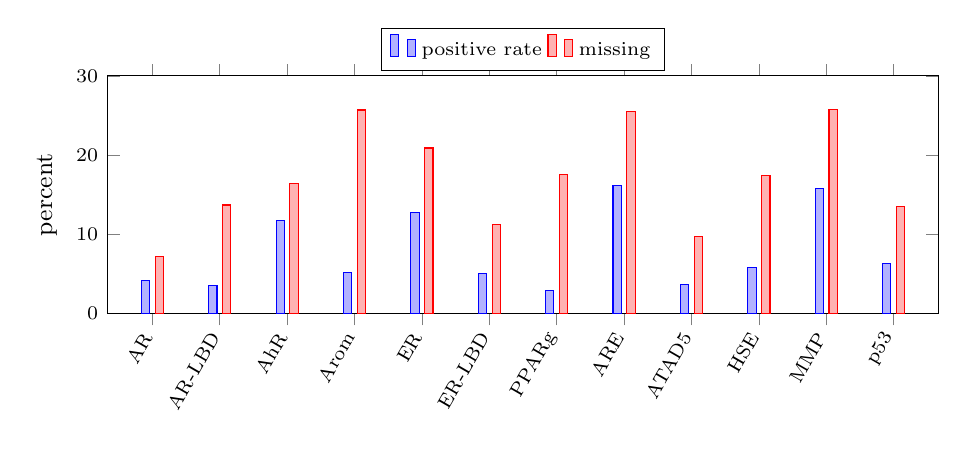
\begin{tikzpicture}
\begin{axis}[ybar, width=\columnwidth, height=4.6cm, bar width=3pt, ymin=0, ymax=30,
 symbolic x coords={AR,AR-LBD,AhR,Arom,ER,ER-LBD,PPARg,ARE,ATAD5,HSE,MMP,p53},
 xtick=data, x tick label style={rotate=60,anchor=east,font=\scriptsize}, ylabel={percent}, ylabel style={font=\small},
 legend style={font=\scriptsize, at={(0.5,1.02)}, anchor=south, legend columns=2}, enlarge x limits=0.06, tick label style={font=\scriptsize}]
\addplot coordinates {(AR,4.2)(AR-LBD,3.5)(AhR,11.7)(Arom,5.2)(ER,12.8)(ER-LBD,5.0)(PPARg,2.9)(ARE,16.2)(ATAD5,3.7)(HSE,5.8)(MMP,15.8)(p53,6.3)};
\addplot coordinates {(AR,7.2)(AR-LBD,13.7)(AhR,16.4)(Arom,25.7)(ER,20.9)(ER-LBD,11.2)(PPARg,17.6)(ARE,25.5)(ATAD5,9.7)(HSE,17.4)(MMP,25.8)(p53,13.5)};
\legend{positive rate, missing}
\end{axis}
\end{tikzpicture}
\caption{Positive rate (of labeled entries) and missing fraction per endpoint.}\label{fig:balance}
\end{figure}

\section{Exploratory Data Analysis}
\textbf{Methods.} For endpoints $i,j$ on molecules labeled for both, with counts $n_{ab}$ of $(y_i,y_j)=(a,b)$, the phi coefficient is $\phi=\frac{n_{11}n_{00}-n_{10}n_{01}}{\sqrt{(n_{11}+n_{10})(n_{01}+n_{00})(n_{11}+n_{01})(n_{10}+n_{00})}}$ and the mutual information is $\sum_{a,b}\frac{n_{ab}}{N}\log_2\frac{n_{ab}N}{n_{a\cdot}n_{\cdot b}}$; both were computed for all endpoint pairs and saved with the code. Morgan bit fingerprints (radius 2, 2048 bits) form $X\in\{0,1\}^{n\times d}$. PCA uses the SVD $X_c=USV^\top$ of the centered matrix, with component variance $s_k^2/(n-1)$. Similarity is the Tanimoto coefficient $T(a,b)=c/(|a|+|b|-c)$, $c=|a\wedge b|$~\cite{bajusz2015tanimoto}. Scaffold diversity is the entropy $H=-\sum_s p_s\log_2p_s$ and the effective number of scaffolds $2^H$.

\textbf{Results.} The first three principal components explain only 4.1\%, 3.3\% and 2.8\% of the variance, and 815 components are needed for 90\%: the fingerprint space has no low-dimensional structure and is high-dimensional and sparse. The mean nearest-neighbor Tanimoto similarity is 0.607 (median 0.600), and 28.2\% of molecules have a neighbor above 0.7, while the mean pairwise distance $1-T$, estimated on a random subsample of 2{,}000 molecules, is 0.919. The set is therefore diverse overall but contains many close analogues, which is why random splits overstate performance. There are 2{,}325 distinct scaffolds, but the effective number is only 163.6 ($H\approx7.35$ bits), so the distribution is very uneven: the largest group alone holds 1{,}775 molecules (22.7\%). This matters for splitting (Section~\ref{sec:theory}).

\section{Feature Engineering}
\textbf{Implemented.} Morgan bit fingerprints (radius 2, 2048 bits) are the only features used so far.

\textbf{Designed for the next stage.} (i) Ten RDKit descriptors (molecular weight, logP, polar surface area, hydrogen-bond donors and acceptors, rotatable bonds, ring count, aromatic rings, $sp^3$ fraction, heteroatoms) capturing size, lipophilicity and polarity. (ii) Eight SMARTS structural alerts (Michael acceptor, aromatic amine, epoxide, aromatic nitro, acyl halide, azo, aldehyde, alkyl halide) as an interpretable expert signal. (iii) Graph features: a 21-dimensional atom vector (atom type, atomic number, acceptor/donor, aromaticity, hybridization, hydrogens, degree) and a 5-dimensional bond one-hot, with each bond as two directed edges. Descriptors would be standardized with training-split statistics only, to avoid leakage.

\textbf{Motivation from the analysis.} The linear model below has $2048\times12+12=24{,}588$ parameters for about 6{,}300 training molecules, PCA shows no compact fingerprint subspace, and the baseline overfits strongly (Table~\ref{tab:baseline}). Low-dimensional descriptors and alerts, and a learned graph embedding, are the natural ways to add information without adding that many free parameters; their value will be measured by ablation (fingerprint only, descriptors only, graph only, fusion).

\section{Theoretical Foundations}\label{sec:theory}
\textbf{Masked loss.} Let $y_{it}\in\{0,1\}$ be observed only when $m_{it}=1$, with logits $z_{it}$ and $p_{it}=\sigmoid(z_{it})$. With $\ell(z,y)=\log(1+e^{z})-yz$,
\begin{equation}
\mathcal L=\frac{\sum_{i,t}m_{it}\,\ell(z_{it},y_{it})}{\sum_{i,t}m_{it}},\qquad \frac{\partial\ell}{\partial z}=\sigmoid(z)-y,
\end{equation}
so missing entries add neither loss nor gradient. $\ell$ is convex in $z$, hence the loss is convex for linear models. The linear multitask model $z_{it}=w_t^\top x_i+b_t$ is mathematically twelve independent logistic regressions trained together; real multitask sharing needs a shared hidden layer.

\textbf{Optimizers.} With gradient $g_t$ and rate $\eta$: RMSprop uses $v_t=\alpha v_{t-1}+(1-\alpha)g_t^2$ and $\theta\leftarrow\theta-\eta g_t/(\sqrt{v_t}+\epsilon)$, a per-parameter step size, which helps rarely active fingerprint bits. Adam~\cite{kingma2015adam} keeps $m_t=\beta_1m_{t-1}+(1-\beta_1)g_t$ and $v_t$ with $\beta_2$, and corrects the start-up bias of the zero initialization: if the gradient has constant mean, $\mathbb E[m_t]=(1-\beta_1^t)\mathbb E[g]$, so $\hat m_t=m_t/(1-\beta_1^t)$ and $\theta\leftarrow\theta-\eta\hat m_t/(\sqrt{\hat v_t}+\epsilon)$; the first step is about $\eta\,\mathrm{sign}(g)$. AdamW~\cite{loshchilov2019adamw} decays weights directly, $\theta\leftarrow\theta(1-\eta\lambda)$, instead of adding $\lambda\theta$ to the gradient, where Adam would divide it by $\sqrt{\hat v_t}$. With $\eta=10^{-3}$ and $\lambda=10^{-2}$ the decay factor is $1-10^{-5}$ per step, so AdamW and Adam behave almost identically here. The optimizers were written from the update equations and checked numerically against \texttt{torch.optim}~\cite{paszke2019pytorch}.

\textbf{Imbalance and metrics.} Weighting positives by $w=n^-/n^+$ moves the minimizer's odds to $w\,\eta/(1-\eta)$, $\eta=P(y{=}1\mid x)$: ranking is kept, probabilities are inflated. ROC-AUC equals $P(s^+>s^-)+\tfrac12P(s^+=s^-)$ and is threshold-free; average precision (PR-AUC) is more informative when positives are rare~\cite{saito2015pr}. Precision, recall and $F_1=2PR/(P+R)$ depend on a threshold, chosen on validation data. We also report $R^2$ of the probabilities against the labels; because $\mathrm{Var}(y)=\bar y(1-\bar y)$ for binary $y$, $R^2=1-\mathrm{BS}/(\bar y(1-\bar y))$ with $\mathrm{BS}$ the Brier score, a skill score against the base rate that can be negative. Metrics are computed per endpoint on labeled entries and averaged over endpoints where defined.

\textbf{Message passing and fusion (planned).} Node states follow $m_v^{t+1}=\sum_{w\in\mathcal N(v)}A(e_{vw})h_w^t$ with $A$ an MLP producing a $d\times d$ matrix from the bond features, and $h_v^{t+1}=\mathrm{GRU}(h_v^t,m_v^{t+1})$~\cite{gilmer2017mpnn}. A Set2Set readout~\cite{vinyals2016order} yields a graph embedding $g\in\mathbb R^{2d}$ by iterating $q_s=\mathrm{LSTM}(q^*_{s-1})$, $a_{i,s}=\mathrm{softmax}_i\langle h_i,q_s\rangle$, $q^*_s=[q_s\Vert\sum_ia_{i,s}h_i]$, which is invariant to node order. Because $A(e)$ is a $d\times d$ matrix per edge, a round costs $O(|E|d^2)$ memory. Fusion concatenates $g$ with an encoded flat feature vector $u$ and applies an MLP head to $[g\Vert u]$.

\textbf{Scaffold splitting.} Assigning whole scaffold groups to one side prevents near-duplicates from leaking. The common greedy procedure shuffles groups and fills train, validation, test in order; with one group holding 22.7\% of the data, the outcome depends on the seed. Under seed 0 on this data the largest group (1{,}775 molecules) was placed entirely in the test set, leaving validation empty; its positive rate was 0.031 against 0.090 in the training set, a large difference between groups. Placing groups larger than half the validation or test target first (so they go to train), then shuffling the rest, removes this failure; we use this balanced rule from now on. With five seeds, an exact two-sided Wilcoxon test cannot give $p<0.0625$, so comparisons will use per-seed paired differences and bootstrap intervals over test molecules rather than significance claims.

\textbf{Calibration.} With $\beta=1/T$, the validation negative log-likelihood of temperature scaling, $\sum_i[\log(1+e^{\beta z_i})-y_i\beta z_i]$, has second derivative $\sum_i\sigmoid'(\beta z_i)z_i^2\ge0$, so it is convex with a unique minimum; dividing logits by $T>0$ keeps their order, so ROC-AUC and PR-AUC are unchanged~\cite{guo2017calibration}.

\section{Model Application and Results}
\textbf{Protocol.} A multitask linear classifier on Morgan bits is trained in mini-batches of 256 molecules with masked cross-entropy. The optimizer is chosen by training each candidate for 15 epochs at its default rate and keeping the lowest validation loss; the number of epochs is chosen by early stopping (patience 15, at most 300), keeping the best-epoch weights; the decision threshold is the value maximizing mean $F_1$ on validation. The test split is used for no choice. The split is a scaffold split with seed 80 using the shuffled greedy procedure (6{,}258 / 782 / 783 molecules for train / validation / test).

\textbf{Optimizer choice.} Validation loss after 15 epochs was 0.3426 for SGD with momentum, 0.3015 for RMSprop, 0.3156 for Adam and 0.3156 for AdamW; RMSprop was selected (rate $10^{-3}$). A 15-epoch budget favors optimizers that start quickly, so this is a choice for the baseline rather than a ranking. Adam and AdamW coincide for the reason given above. Training ran 43 epochs and stopped early; the best epoch was 28 (validation loss 0.2910).

\begin{table}[t]
\centering\small
\caption{Baseline metrics, mean over endpoints (threshold 0.25). ``All'' pools train, validation and test and includes training data. Single scaffold split (seed 80), single run: preliminary.}\label{tab:baseline}
\begin{tabular}{@{}lcccc@{}}
\toprule
Metric & Train & Val & Test & All \\
\midrule
Accuracy & 0.9353 & 0.8834 & 0.8837 & 0.9256 \\
Precision & 0.5286 & 0.4023 & 0.3186 & 0.5199 \\
Recall & 0.5234 & 0.3865 & 0.2762 & 0.4924 \\
$F_1$ & 0.5163 & 0.3896 & 0.2849 & 0.4961 \\
ROC-AUC & 0.9023 & 0.7274 & 0.6539 & 0.8539 \\
PR-AUC & 0.5650 & 0.4160 & 0.2883 & 0.5239 \\
$R^2$ & 0.3080 & 0.1844 & 0.0793 & 0.2815 \\
\bottomrule
\end{tabular}
\end{table}

\textbf{Discussion.} Table~\ref{tab:baseline} shows strong overfitting: ROC-AUC falls from 0.902 on training data to 0.727 on validation and 0.654 on test, and PR-AUC from 0.565 to 0.288. Accuracy is 0.884 on test while $F_1$ is 0.285, which shows why accuracy is the wrong yardstick at these positive rates. The test $R^2$ of 0.079 means the probabilities are barely better than the base rate. The validation--test gap (0.727 vs 0.654) also shows how much results depend on which scaffolds fall in a split; one seed cannot separate that from model quality. These are single-run figures, so differences of a few points should not be interpreted.

\textbf{Planned evaluation.} Random forest, XGBoost~\cite{breiman2001rf,chen2016xgboost}, a GIN baseline, the message-passing network and the fusion model will be compared on the balanced scaffold split with five seeds, reporting mean $\pm$ standard deviation and per-endpoint results, with the feature ablation above and calibration with temperature scaling.

\section{Implementation and Validation}
The code is a Python package with a command-line interface, a lock file and a pinned Python version; \texttt{uv} is used with a \texttt{pip} fallback. The pipeline ran on the real data (cleaning, label summary, analysis, training). The numerical code is tested against independent references: the optimizers match \texttt{torch.optim} for ten configurations; phi, mutual information and PCA match pandas and scikit-learn~\cite{pedregosa2011sklearn}; Tanimoto similarity matches RDKit; and closed-form properties are checked. Two defects were found when running on real data and fixed: a table-formatting crash under pandas~3, and the scaffold-split failure described above, whose fix was verified by simulation on a group-size distribution matching this data (no empty validation set over 50 seeds, sizes within 0.01\% of 80/10/10, against 17 of 50 seeds with an empty validation set for the greedy procedure).

\section{Limitations and Conclusion}
Labels are noisy in-vitro outcomes and the endpoints do not measure human toxicity, so predictions must not be used for safety decisions. The reported baseline is one split and one seed, and only fingerprint features have been implemented. The analysis shows an imbalanced, partly unlabeled, structurally clustered dataset in which a high-dimensional fingerprint model overfits quickly. The next steps are the descriptor, alert and graph features, the baselines and the message-passing and fusion models on five balanced scaffold splits.

\bibliographystyle{IEEEtran}
\bibliography{references}

\end{document}